\documentclass[9pt,t]{beamer}
\graphicspath{{figures/}} % Setting the graphicspath

% Theme settings
\usetheme{Madrid}
\usecolortheme{default}
\setbeamertemplate{navigation symbols}{}   % removes navigation symbols such as 'next page'
\setbeamertemplate{footline}{}             % remove line with name, date, page nr. 
\setbeamercolor*{frametitle}{bg=white}     % remove background from frametitle
\usepackage{caption}
% \captionsetup[figure]{labelformat=empty}% redefines the caption setup of the figures environment in the beamer class.
\setbeamersize{text margin left=20pt,text margin right=10pt}

\usefonttheme[onlymath]{serif} % makes beamer math look like article math


%======================= import packages =======================================
\usepackage{hyperref}
% \usepackage{enumitem}




%======================= page numbering =======================
% \addtobeamertemplate{navigation symbols}{}{ \usebeamerfont{footline}
%   \insertframenumber / \inserttotalframenumber \hspace*{2mm} \\ \vspace*{1mm} 
% }


%=================================== colors ====================================
\definecolor{RoyBlue}{RGB}{22, 46, 69}
\definecolor{RoyGrey}{RGB}{64, 88, 128} 

\newcommand{\hlme}[1]{{\color{red}\bf #1}} % highlight me

\setbeamercolor{structure}{fg=RoyBlue} % itemize, enumerate, etc
\setbeamercolor{frametitle}{fg=RoyGrey}
\setbeamercolor{section in head/foot}{bg=RoyBlue}


%======================= add progress dots to headline =========================
% \setbeamertemplate{headline}{%
%     \begin{beamercolorbox}[ht=4mm,dp=4mm]{section in head/foot}
%         \insertnavigation{\paperwidth}
%     \end{beamercolorbox}%
% }%
% \makeatother


%======================= add section title page ================================
\AtBeginSection[]{
  \begin{frame}
  \vfill
  \centering
    \usebeamerfont{title}\insertsection\par%
  \vfill
  \end{frame}
}


%=================================== titlepage =================================
\title{Preparation for the tutorials}
\date{Advanced Artificial Intelligence \\ for precision High Energy Physics \\[0.1cm] 17 July 2023}

\author{Roy Stegeman}
\institute{The Higgs Centre for Theoretical Physcis, University of Edinburgh}

\titlegraphic{\vspace*{6mm}
	
\includegraphics[height=1.5cm]{logos/edi_logo.png} \hspace{10mm}
	
\includegraphics[height=0.8cm]{logos/nnpdf_logo_official.pdf} \hspace{10mm}
	
\includegraphics[height=1.5cm]{logos/higgs_logo.jpg}
}

\defbeamertemplate{title page}{noinstitute}[1][]
{
  \vbox{}
  \vfill
  \begingroup
    \centering
    \begin{beamercolorbox}[sep=8pt,center,#1]{title}
      \usebeamerfont{title}\inserttitle\par%
      \ifx\insertsubtitle\@empty%
      \else%
        \vskip0.25em%
        {\usebeamerfont{subtitle}\usebeamercolor[fg]{subtitle}\insertsubtitle\par}%
      \fi%     
    \end{beamercolorbox}%
    \vskip1em\par
    \begin{beamercolorbox}[sep=0pt,center,#1]{author}
      \usebeamerfont{author}\insertauthor
    \end{beamercolorbox}
	\begin{beamercolorbox}[sep=0pt,center,#1]{author}
		\usebeamerfont{institute}\insertinstitute
	\end{beamercolorbox}
	\vspace*{8pt}
	\vspace*{16pt}
    \begin{beamercolorbox}[sep=0pt,center,#1]{date}
      \usebeamerfont{date}\insertdate
    \end{beamercolorbox}\vskip0.5em
    {\usebeamercolor[fg]{titlegraphic}\inserttitlegraphic\par}
  \endgroup
  \vfill
}

% \makeatletter
% \setbeamertemplate{title page}[noinstitute][colsep=-4bp,rounded=true,shadow=\beamer@themerounded@shadow]
% \makeatother


\begin{document}

{
\setbeamertemplate{headline}{} % remove headline from titlepage
\begin{frame}
  \titlepage
\end{frame}
}

\setbeamertemplate{enumerate items}[default]

\pgfdeclarelayer{bg}    % declare background layer
\pgfsetlayers{bg,main}  % set the order of the layers (main is the standard layer)


% SLIDES =======================================================================

\begin{frame}{General remarks}
  \vspace*{1cm}
  We have to leave the villa at 1800 each day \\
  \vspace*{1cm}
  The villa cannot be accessed during the weekend, though Milan is only a 40 minute train ride away!
\end{frame}

\begin{frame}{Schedule}
  \begin{columns}
    \begin{column}{0.5\textwidth}
      \textbf{Week 1}\\[1em]
      \textbf{Lecture topics:}
      \begin{itemize}
        \item Quantum Chromodynamics
        \item Machine Learning techniques
      \end{itemize}
      \textbf{Tutorial topics:}
      \begin{enumerate}
        \item Code installation
        \item (NLO) theory predictions
        \item DGLAP evolution
        \item ML 101: regression and classification
        \item ML for HEP (jets and PDFs)
      \end{enumerate}
    \end{column}
    \begin{column}{0.5\textwidth}
      \textbf{Week 2}\\[1em]
      \textbf{Lecture topics:}
      \begin{itemize}
        \item Bayesian methods and data analysis
        \item Quantum Machine Learning
      \end{itemize}
      \textbf{Tutorial topics:}

      \begin{enumerate}
        \item Bayesian inference tools
        \item Quantum Computing
        \item Quantum Machine Learning
        \item Exercise: SM Bayesian fit
        \item No tutorial on Friday
      \end{enumerate}
    \end{column}
  \end{columns}
\end{frame}

\begin{frame}{Factorization: a quick reminder}

  \begin{columns}
    \begin{column}{0.5\textwidth}
      \textbf{High-energy scattering experiments} such as performed at the LHC involves processes with \textbf{hadrons in the initial state}
    \end{column}
    \begin{column}{0.5\textwidth}
      \vspace*{-1cm}
      \begin{figure}
        \centering
        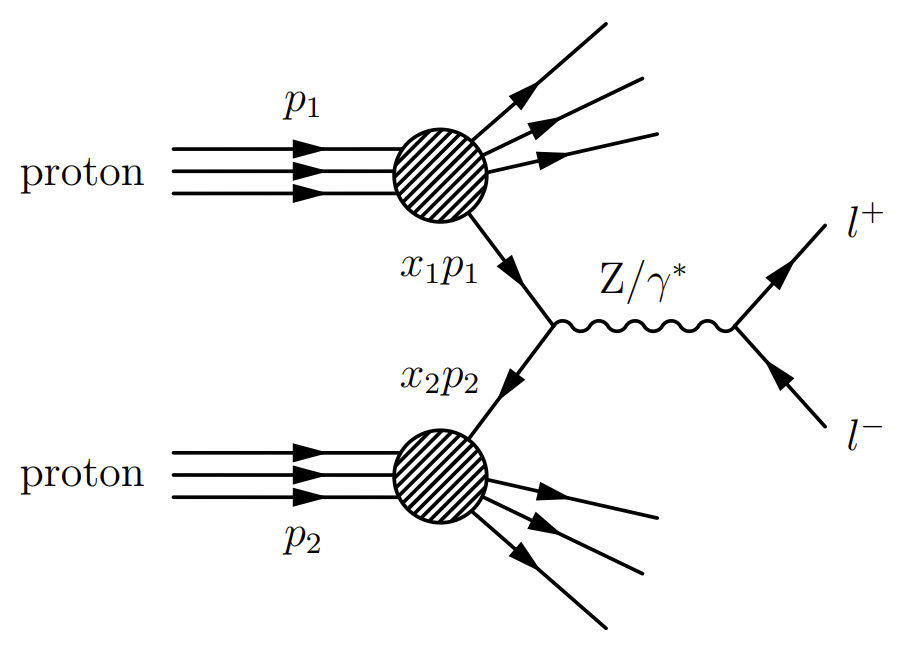
\includegraphics[width=0.8\textwidth]{figures/dy.png}
      \end{figure}
    \end{column}
  \end{columns}


  Total cross-section is \textbf{factorized} into a \textcolor{red}{hard part, $\hat{\sigma}$}, and process-independent \textcolor{blue}{parton distribution functions (PDFs), $f_{i/h}$}, providing the distribution of partons inside the hadron $h$:
  $$
    \sigma=\sum_{i, j} \int_0^1 \mathrm{~d} x_1 \mathrm{~d} x_2 \textcolor{blue}{f_{i / h_1}\left(x_1, \mu_F^2\right) f_{j / h_2}\left(x_2, \mu_F^2\right)} \textcolor{red}{\hat{\sigma}_{i j \rightarrow X }(x_1p_1, x_2p_2, \mu_F^2)}
  $$

  \vspace*{1cm}
  \begin{center}
    \textbf{How are PDFs determined?}
  \end{center}

\end{frame}



\begin{frame}{PDF determination}
  \begin{figure}
    \centering
    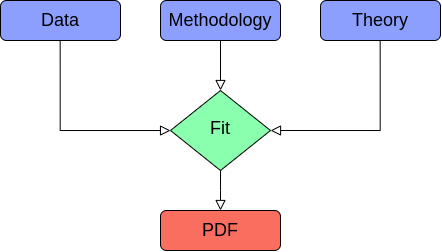
\includegraphics[width=0.6\textwidth]{figures/pdffitflowchart.png}
  \end{figure}
  \begin{itemize}
    \item \textbf{Theory}: partonic cross-sections and DGLAP (Tuesday and Wednesday)
    \item \textbf{Methodology}: regression and neural nets (Thursday and Friday)
    \item \textbf{Data}: From experiments
  \end{itemize}
\end{frame}



\begin{frame}{Preparing your laptops}
  Requirements as stated in the e-mail:
  \begin{itemize}
    \item Ubuntu 20.04 or higher / macOS 11 or higher
    \item Working LHAPDF installation (hopefully)
    \item Python 3.8, 3.9, or 3.10 
  \end{itemize}
  \vspace*{0.5cm}
  The goal for this afternoon is to set up the environments for the next two weeks
\end{frame}


\begin{frame}[containsverbatim]{Preparing your laptops}
  \begin{enumerate}
    \item Clone/download the repository \url{https://github.com/NNPDF/como-2023}
    \item Set up the environments
    \begin{itemize}
      \item This can be done by initializing a virtual environment (in this case \textcolor{gray}{theory}) using\\
      \hspace*{0.5cm}\textcolor{gray}{\$ python -m venv \$REPO/envs/theory} \\
      then activating it: \\ 
      \hspace*{0.5cm}\textcolor{gray}{\$ source \$REPO/envs/theory/bin/activate} \\
      and finally install the required packages: \\
      \hspace*{0.5cm}\textcolor{gray}{\$ pip install -r \$REPO/envs/theory/requirements.txt} \\
      Alternative environment managers are also fine
      \item If you used conda to install LHAPDF, you can use this environment as the machine learning (\textcolor{gray}{ml}) and \textcolor{gray}{theory} environments: \\
      \hspace*{0.5cm}\textcolor{gray}{\$ conda install -{}-file \$REPO/envs/ml/requirements.txt}
      \item Make sure the LHAPDF installation can be found inside your environments paths
    \end{itemize}
    \item Test the environments by running example notebooks \\
    \hspace*{0.5cm}\textcolor{gray}{\$ jupyter lab [jupyter notebook]}
    \item To save time tomorrow we can compile \textcolor{gray}{eko} ahead of time by running \\
    \hspace*{0.5cm}\textcolor{gray}{\$ python Como-2023/w1t3-rge-pdfs/compile.py}

  \end{enumerate}
  \vspace*{0.6cm}
  \begin{center}
    \textbf{If this is successful, we'll see you again tomorrow!}
  \end{center}
\end{frame}





\end{document}
